\section{Manager Class Reference}
\label{classManager}\index{Manager@{Manager}}
{\tt \#include $<$manager.h$>$}

Inheritance diagram for Manager:\nopagebreak
\begin{figure}[H]
\begin{center}
\leavevmode
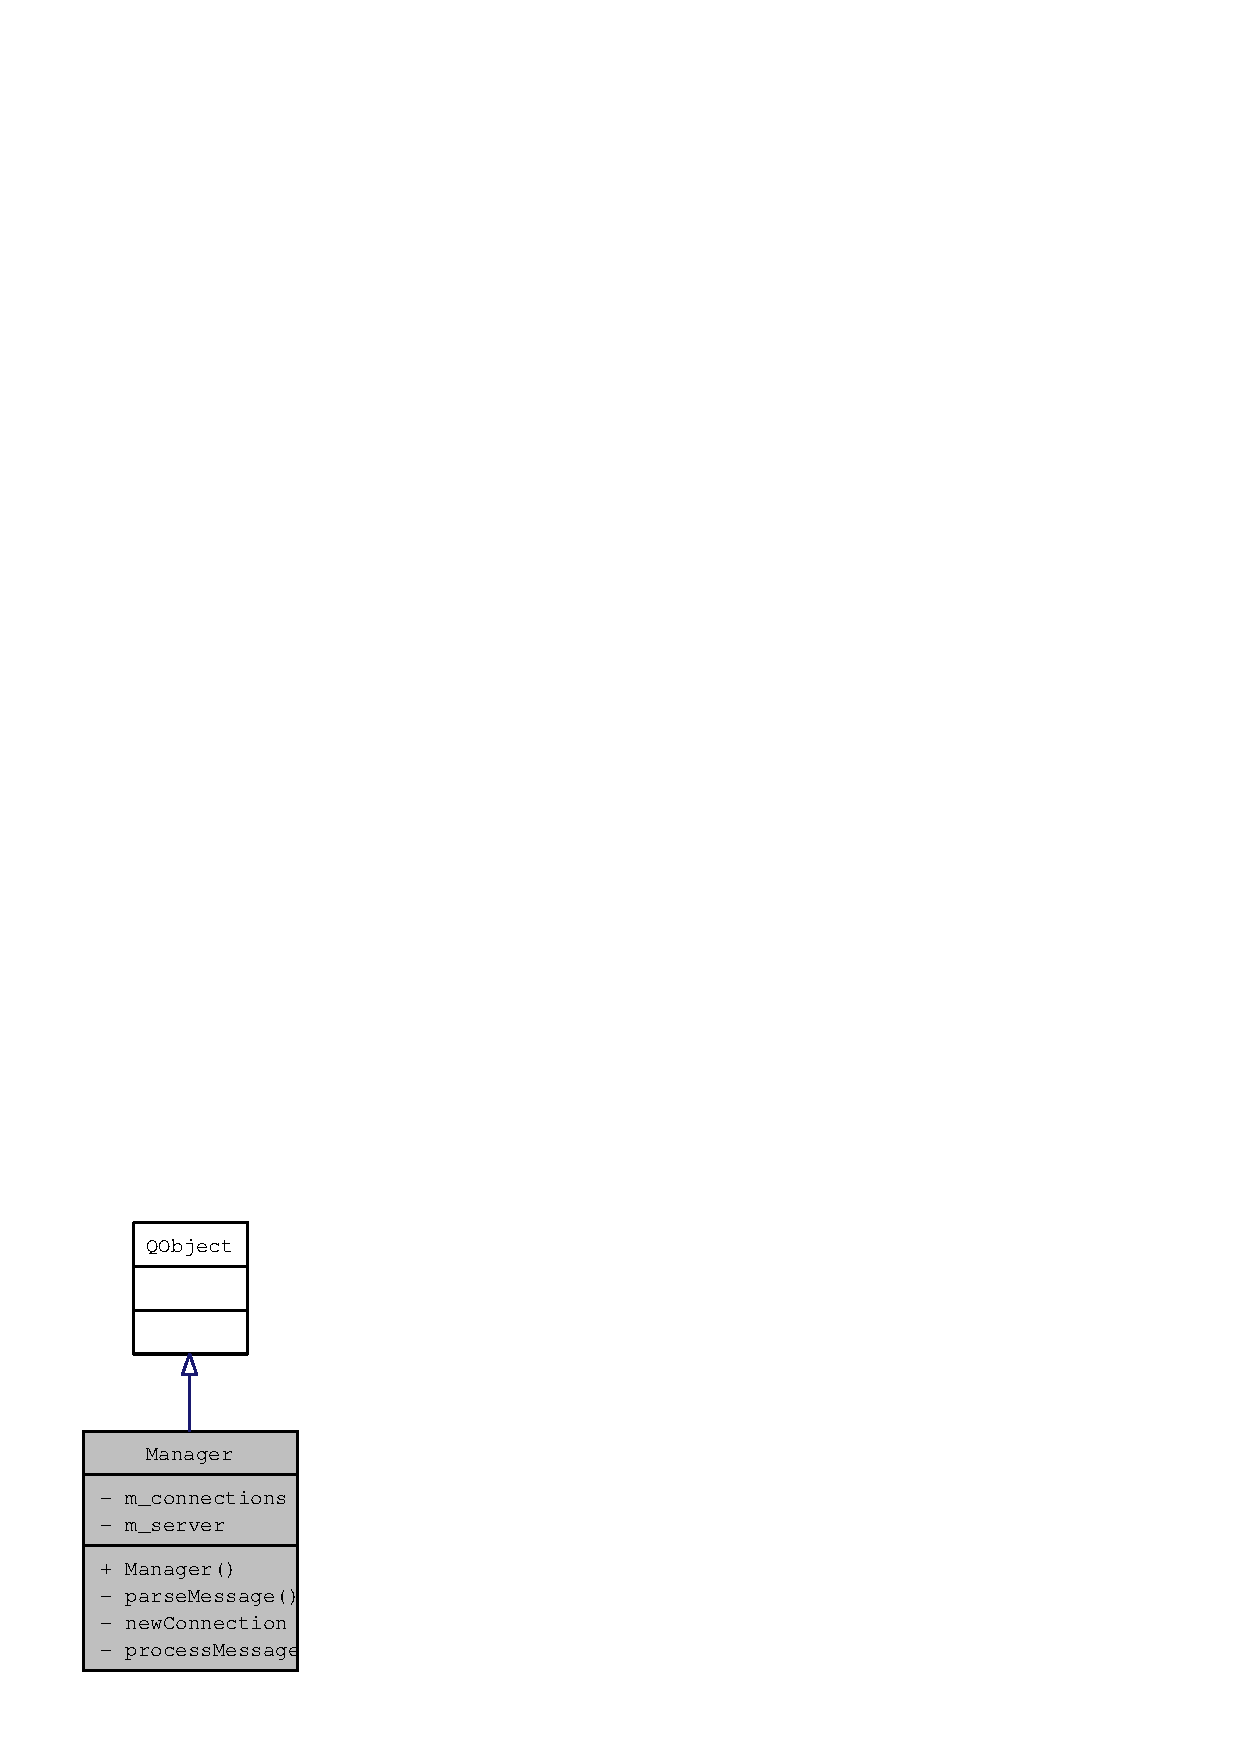
\includegraphics[width=73pt]{classManager__inherit__graph}
\end{center}
\end{figure}
Collaboration diagram for Manager:\nopagebreak
\begin{figure}[H]
\begin{center}
\leavevmode
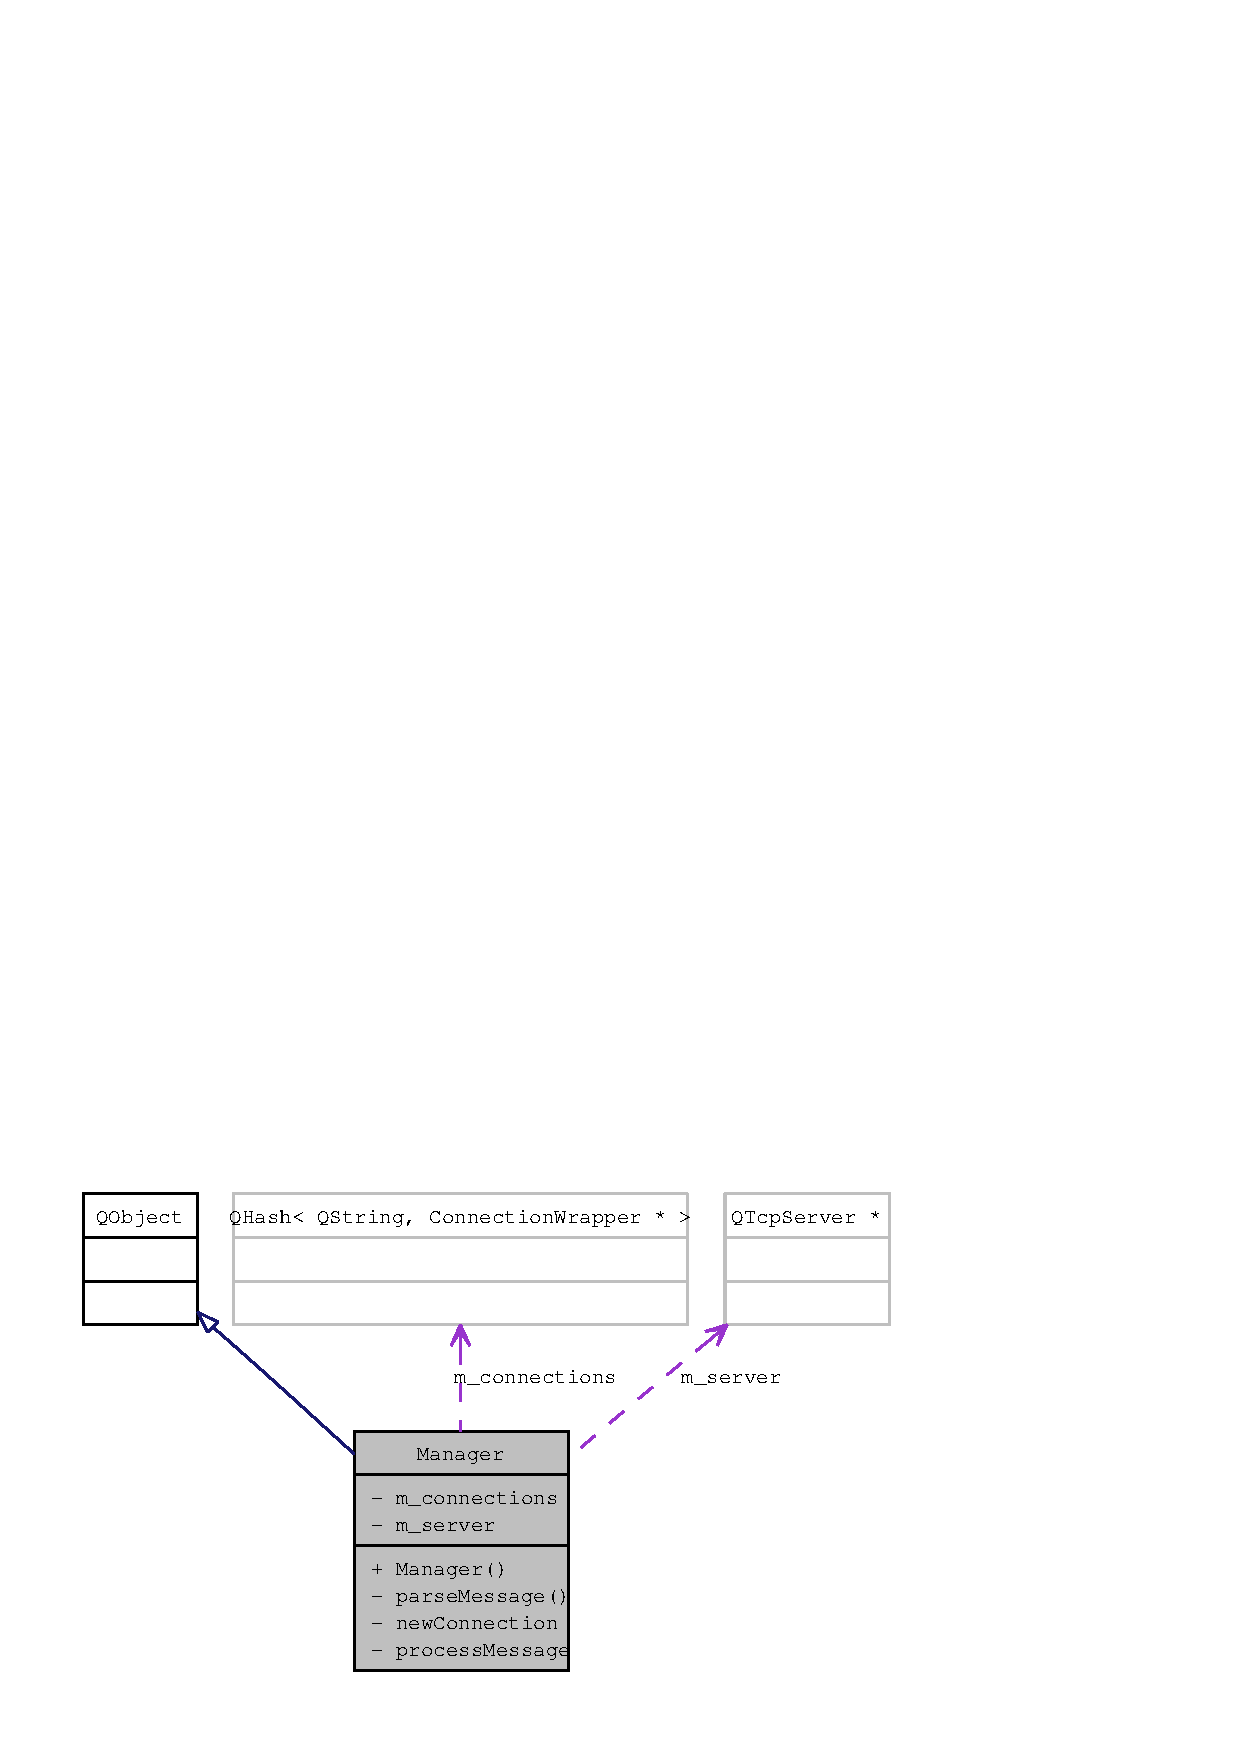
\includegraphics[width=400pt]{classManager__coll__graph}
\end{center}
\end{figure}
\subsection*{Signals}
\begin{CompactItemize}
\item 
void {\bf message} (const QString \&message)
\end{CompactItemize}
\subsection*{Public Member Functions}
\begin{CompactItemize}
\item 
{\bf Manager} ({\bf QTcpServer} $\ast$server, {\bf QObject} $\ast$parent=0)
\end{CompactItemize}
\subsection*{Private Slots}
\begin{CompactItemize}
\item 
void {\bf newConnection} ()
\item 
void {\bf processMessage} (const QString \&message)
\end{CompactItemize}
\subsection*{Private Member Functions}
\begin{CompactItemize}
\item 
QString {\bf parseMessage} (const QString \&m, QStringList $\ast$tokens)
\end{CompactItemize}
\subsection*{Private Attributes}
\begin{CompactItemize}
\item 
QHash$<$ QString, {\bf ConnectionWrapper} $\ast$ $>$ {\bf m\_\-connections}
\item 
{\bf QTcpServer} $\ast$ {\bf m\_\-server}
\end{CompactItemize}


\subsection{Detailed Description}


Definition at line 9 of file manager.h.

\subsection{Constructor \& Destructor Documentation}
\index{Manager@{Manager}!Manager@{Manager}}
\index{Manager@{Manager}!Manager@{Manager}}
\subsubsection{\setlength{\rightskip}{0pt plus 5cm}Manager::Manager ({\bf QTcpServer} $\ast$ {\em server}, {\bf QObject} $\ast$ {\em parent} = {\tt 0})}\label{classManager_19000c19438e7e30381ed764ac4ef61a}




Definition at line 8 of file manager.cpp.

References m\_\-server, and newConnection().

\begin{Code}\begin{verbatim}9         :QObject(parent), m_server(server)
10 {
11     connect(m_server, SIGNAL(newConnection()),
12             this, SLOT(newConnection()));
13 }
\end{verbatim}
\end{Code}




\subsection{Member Function Documentation}
\index{Manager@{Manager}!message@{message}}
\index{message@{message}!Manager@{Manager}}
\subsubsection{\setlength{\rightskip}{0pt plus 5cm}void Manager::message (const QString \& {\em message})\hspace{0.3cm}{\tt  [signal]}}\label{classManager_5d591fad4739498d9b9dd0bdcaaebfc3}




Referenced by newConnection(), and processMessage().\index{Manager@{Manager}!newConnection@{newConnection}}
\index{newConnection@{newConnection}!Manager@{Manager}}
\subsubsection{\setlength{\rightskip}{0pt plus 5cm}void Manager::newConnection ()\hspace{0.3cm}{\tt  [private, slot]}}\label{classManager_e7859713b4091f38ab52ad73c18fb2d2}




Definition at line 15 of file manager.cpp.

References m\_\-server, message(), and processMessage().

Referenced by Manager().

\begin{Code}\begin{verbatim}16 {
17     if (m_server->hasPendingConnections()) {
18         QTcpSocket* socket = m_server->nextPendingConnection();
19         ConnectionWrapper* w = new ConnectionWrapper(socket, this);
20         connect(w, SIGNAL(gotMessage(QString)),
21                 this, SLOT(processMessage(QString)));
22         connect(this, SIGNAL(message(QString)),
23                 w, SLOT(sendMessage(QString)));
24     }
25 }
\end{verbatim}
\end{Code}


\index{Manager@{Manager}!parseMessage@{parseMessage}}
\index{parseMessage@{parseMessage}!Manager@{Manager}}
\subsubsection{\setlength{\rightskip}{0pt plus 5cm}QString Manager::parseMessage (const QString \& {\em m}, QStringList $\ast$ {\em tokens})\hspace{0.3cm}{\tt  [private]}}\label{classManager_2650eab19167d3fa4a114d614c84d759}




Definition at line 69 of file manager.cpp.

Referenced by processMessage().

\begin{Code}\begin{verbatim}70 {
71     tokens->clear();
72 
73     QStringList words = m.split(" ");
74     if (words.count() == 0)
75         return QString();
76 
77     QString command = words.takeAt(0).toUpper();
78     if (command == "NICK") { // NICK knows 2 arguments so take first 2
79         for (int i = 0; i < 2 && words.count() != 0; i++) {
80             tokens->append(words.takeAt(0));
81         }
82         return command;
83     } else if (command == "SAY") {
84         if (words.count() >= 2) { // SAY has 2 real arguments but n words
85             tokens->append(words.takeAt(0));
86             tokens->append(words.join(" "));
87             return command;
88         }
89     }
90 
91     return QString();
92 }
\end{verbatim}
\end{Code}


\index{Manager@{Manager}!processMessage@{processMessage}}
\index{processMessage@{processMessage}!Manager@{Manager}}
\subsubsection{\setlength{\rightskip}{0pt plus 5cm}void Manager::processMessage (const QString \& {\em message})\hspace{0.3cm}{\tt  [private, slot]}}\label{classManager_6c73fe4165b0bba176d9177812d9407a}




Definition at line 27 of file manager.cpp.

References ConnectionWrapper::isRegistered(), m\_\-connections, message(), ConnectionWrapper::nick(), parseMessage(), ConnectionWrapper::sendMessage(), ConnectionWrapper::setNick(), and ConnectionWrapper::setRegistered().

Referenced by newConnection().

\begin{Code}\begin{verbatim}28 {
29     ConnectionWrapper* c = qobject_cast<ConnectionWrapper*>(sender());
30     Q_ASSERT(c);
31 
32     QString m = msg.trimmed();
33     QString type;
34     QStringList tokens;
35     
36     qDebug() << m;
37     
38     type = parseMessage(m, &tokens);
39     if (type.isNull()) {
40         qDebug() << "Received invalid command!";
41         return;
42     }
43 
44     // For unregistered connections only NICK command is supported...
45     if (type == "NICK") {
46         QString nick = tokens[0];
47         if (c->isRegistered()) {
48             emit message(QString("NICK %1 %2").arg(nick).arg(c->nick()));
49         } else if (!c->isRegistered()){
50             c->sendMessage(QString("NICK %1").arg(nick));
51             m_connections[nick] = c;
52             c->setRegistered(true);
53             emit message(QString("STATUS %1 is now connected.").arg(nick));
54         }
55         c->setNick(nick);
56     }
57 
58     // ... but registered connections get the whole shebang, so bail now
59     // if the connection has not yet registered.
60     if (!c->isRegistered())
61         return;
62 
63     if (type == "SAY") {
64         QString toks = tokens.join(" ");
65         emit message(QString("SAY %1").arg(toks));
66     }
67 }
\end{verbatim}
\end{Code}




\subsection{Member Data Documentation}
\index{Manager@{Manager}!m_connections@{m\_\-connections}}
\index{m_connections@{m\_\-connections}!Manager@{Manager}}
\subsubsection{\setlength{\rightskip}{0pt plus 5cm}QHash$<$QString, {\bf ConnectionWrapper}$\ast$$>$ {\bf Manager::m\_\-connections}\hspace{0.3cm}{\tt  [private]}}\label{classManager_5a8a686f11fabe55d7ae84990f9e2113}




Definition at line 26 of file manager.h.

Referenced by processMessage().\index{Manager@{Manager}!m_server@{m\_\-server}}
\index{m_server@{m\_\-server}!Manager@{Manager}}
\subsubsection{\setlength{\rightskip}{0pt plus 5cm}{\bf QTcpServer}$\ast$ {\bf Manager::m\_\-server}\hspace{0.3cm}{\tt  [private]}}\label{classManager_5430d52079cf0e14d9d92971f3a229e5}




Definition at line 25 of file manager.h.

Referenced by Manager(), and newConnection().

The documentation for this class was generated from the following files:\begin{CompactItemize}
\item 
{\bf manager.h}\item 
{\bf manager.cpp}\end{CompactItemize}
